\chapter*{ENVIRONNEMENT DE DÉVELOPPEMENT}
\addcontentsline{toc}{chapter}{ENVIRONNEMENT DE DÉVELOPPEMENT}


\section{Prérequis Système}

\subsection{Configuration matérielle requise}

Le développement et l'exécution du système Agriculture Cameroun nécessitent une configuration matérielle adaptée pour garantir des performances optimales et une expérience de développement fluide. Les exigences matérielles ont été soigneusement calibrées pour équilibrer accessibilité et performance, permettant aux développeurs avec des configurations modestes de contribuer au projet tout en assurant une exécution efficace du système complet.

La \textbf{mémoire vive (RAM)} constitue l'élément le plus critique pour le bon fonctionnement du système. Un minimum de \textbf{8 GB de RAM} est requis pour exécuter le système de base avec ses cinq agents spécialisés. Cette capacité permet le chargement des modèles de langage, le maintien des contextes de conversation et l'exécution simultanée de plusieurs agents. Cependant, pour une expérience de développement optimale incluant l'exécution de tests, le débogage et l'utilisation d'outils de développement, \textbf{16 GB de RAM} sont fortement recommandés. Cette configuration supérieure permet également de travailler confortablement avec plusieurs instances du système pour les tests de charge et le développement parallèle.

Le \textbf{processeur} doit être suffisamment puissant pour gérer les opérations intensives de traitement du langage naturel et la coordination multi-agents. Un processeur \emph{quad-core} moderne (Intel Core i5 de 8ème génération ou équivalent AMD Ryzen 5) constitue la configuration minimale. Les processeurs avec plus de cœurs offrent des avantages significatifs pour l'exécution parallèle des agents et l'amélioration des temps de réponse. Les architectures récentes avec support des instructions AVX bénéficient d'optimisations supplémentaires pour les opérations d'intelligence artificielle.

L'\textbf{espace de stockage} nécessaire dépend de l'utilisation prévue du système. Un minimum de \textbf{2 GB d'espace libre} est requis pour l'installation de base du système, incluant le code source, les dépendances Python et les données agricoles locales. Pour un environnement de développement complet avec historique Git, environnements virtuels multiples et données de test étendues, prévoir au moins \textbf{5 GB d'espace libre}. L'utilisation d'un \emph{SSD} plutôt qu'un disque dur traditionnel améliore significativement les temps de chargement et la réactivité générale du système.

La \textbf{connexion Internet} joue un rôle crucial dans le fonctionnement du système. Une connexion \emph{haut débit stable} est indispensable pour l'accès aux API de Google Gemini, le téléchargement des dépendances et la synchronisation avec les dépôts Git. Une bande passante minimale de \textbf{10 Mbps} est recommandée pour une utilisation confortable, avec une latence faible pour optimiser les interactions avec les services cloud. Les développeurs travaillant dans des zones avec connectivité limitée devraient considérer l'implémentation de mécanismes de cache et de mode hors ligne pour certaines fonctionnalités.

La \textbf{carte graphique} n'est pas strictement nécessaire pour l'exécution du système de base, car le traitement principal se fait via les API cloud de Google. Cependant, pour les développeurs souhaitant expérimenter avec des modèles locaux ou implémenter des fonctionnalités de vision par ordinateur pour l'analyse d'images de cultures, une carte graphique avec support CUDA peut être bénéfique.

\subsection{Systèmes d'exploitation supportés}

Le système Agriculture Cameroun a été conçu avec une philosophie de \textbf{compatibilité multiplateforme}, assurant que les développeurs peuvent contribuer indépendamment de leur environnement de travail préféré. Cette approche inclusive maximise le potentiel de collaboration et facilite l'adoption dans différents contextes techniques.

\textbf{Linux} constitue l'environnement de développement privilégié, offrant la meilleure expérience en termes de performance et de compatibilité. Les distributions basées sur \emph{Debian/Ubuntu} (Ubuntu 20.04 LTS et versions ultérieures, Debian 10+) sont particulièrement bien supportées, avec des scripts d'installation automatisés et une documentation extensive. Les distributions basées sur \emph{Red Hat} (Fedora 33+, CentOS 8+, RHEL 8+) sont également pleinement compatibles. L'écosystème Linux offre des avantages significatifs pour le développement, incluant une gestion native des permissions, des outils de développement puissants et une excellente intégration avec les technologies cloud.

\textbf{Windows} est supporté à partir de \emph{Windows 10 version 1903} et versions ultérieures, incluant Windows 11. Le support Windows a été soigneusement implémenté pour assurer une parité fonctionnelle avec Linux. L'utilisation du \emph{Windows Subsystem for Linux (WSL2)} est recommandée pour les développeurs Windows cherchant une expérience plus proche de l'environnement Linux. Les scripts PowerShell fournis automatisent l'installation des composants nécessaires et configurent l'environnement de manière optimale. Les développeurs Windows doivent porter une attention particulière à la gestion des chemins de fichiers et aux différences de fin de ligne dans les fichiers texte.

\textbf{macOS} est supporté à partir de \emph{macOS 10.15 (Catalina)} et versions ultérieures. L'environnement macOS offre un excellent compromis entre l'interface utilisateur conviviale et la puissance des outils Unix sous-jacents. Les développeurs macOS bénéficient de Homebrew pour la gestion simplifiée des dépendances système. Les architectures Intel et Apple Silicon (M1/M2) sont toutes deux supportées, avec des optimisations spécifiques pour tirer parti des performances des puces ARM d'Apple.

Les \textbf{environnements de développement cloud} constituent une option de plus en plus populaire. Le système est compatible avec les principales plateformes cloud de développement comme GitHub Codespaces, Gitpod et Google Cloud Shell. Ces environnements offrent l'avantage d'une configuration standardisée et de ressources scalables, particulièrement utiles pour les développeurs avec des machines locales limitées ou pour la collaboration en équipe.

Pour les \textbf{environnements conteneurisés}, le projet fournit des configurations Docker complètes permettant l'exécution du système dans des conteneurs isolés. Cette approche garantit une cohérence parfaite entre les environnements de développement, de test et de production, éliminant les problèmes classiques de "ça marche sur ma machine". Les images Docker sont optimisées pour minimiser leur taille tout en incluant toutes les dépendances nécessaires.

\subsection{Versions Python et dépendances}

Le choix de \textbf{Python 3.12} comme version minimale requise reflète l'engagement du projet envers l'utilisation des fonctionnalités modernes du langage tout en maintenant une stabilité production. Cette version apporte des améliorations significatives en termes de performance, de syntaxe et de fonctionnalités qui bénéficient directement au développement d'applications d'intelligence artificielle.

Python 3.12 introduit des \emph{optimisations de performance} substantielles, particulièrement bénéfiques pour les applications intensives en traitement de données comme notre système multi-agents. Les améliorations de l'interpréteur CPython résultent en une exécution jusqu'à 25% plus rapide pour certaines opérations, réduisant la latence globale du système. Les nouvelles fonctionnalités de typage, incluant les améliorations des génériques et les types paramétriques, permettent un code plus robuste et maintenable, essentiels pour un projet collaboratif.

La \textbf{gestion des dépendances} est orchestrée par Poetry, offrant une approche moderne et déterministe de la gestion des packages Python. Les dépendances principales du projet incluent \emph{google-generativeai} pour l'intégration avec Gemini, \emph{python-dotenv} pour la gestion sécurisée des variables d'environnement, \emph{pydantic} pour la validation robuste des données, \emph{httpx} pour les requêtes HTTP asynchrones performantes, et \emph{pytest} avec ses plugins pour un framework de test complet.

Les \textbf{dépendances système} varient selon la plateforme mais incluent généralement des compilateurs C/C++ pour certaines extensions Python, des bibliothèques de développement Python (python3-dev sur Linux), et des outils de construction comme make et cmake. Ces dépendances sont généralement gérées automatiquement par les scripts d'installation fournis, mais leur compréhension est importante pour le débogage d'éventuels problèmes d'installation.

La \textbf{compatibilité ascendante} avec les versions Python ultérieures est activement maintenue. Le projet utilise des pratiques de codage qui évitent la dépendance à des fonctionnalités dépréciées et inclut des tests de compatibilité avec les versions bêta de Python. Cette approche proactive assure que le système reste compatible avec les futures versions de Python, protégeant l'investissement en développement.

La \textbf{gestion des environnements virtuels} est cruciale pour maintenir l'isolation des dépendances et éviter les conflits entre projets. Poetry gère automatiquement la création et l'activation des environnements virtuels, assurant que chaque développeur travaille dans un environnement cohérent et reproductible. Cette isolation est particulièrement importante lors du développement de fonctionnalités expérimentales ou du test de nouvelles versions de dépendances.

\section{Installation de l'Environnement}

\subsection{Installation de Python 3.12+}

L'installation de Python constitue la première étape cruciale dans la configuration de l'environnement de développement. La procédure varie selon le système d'exploitation, mais l'objectif reste constant : obtenir une installation Python moderne et correctement configurée.
\subsubsection{Installation sur Windows}

Pour les utilisateurs Windows, l'installation de Python nécessite une attention particulière pour assurer une configuration optimale. Commencez par naviguer vers le site officiel Python à l'adresse \texttt{\href{https://www.python.org/downloads/}{python.org/downloads}}. Le site détecte automatiquement votre système d'exploitation et propose la dernière version stable de Python compatible.

Téléchargez l'installateur Windows 64-bit (ou 32-bit selon votre système). Lors du lancement de l'installateur, l'écran d'accueil présente une option cruciale : \textbf{"Add Python to PATH"}. Il est impératif de cocher cette case avant de procéder à l'installation. Cette action permet d'accéder à Python depuis n'importe quel répertoire dans l'invite de commandes, évitant de nombreux problèmes de configuration ultérieurs.

\begin{figure}[H]
\centering
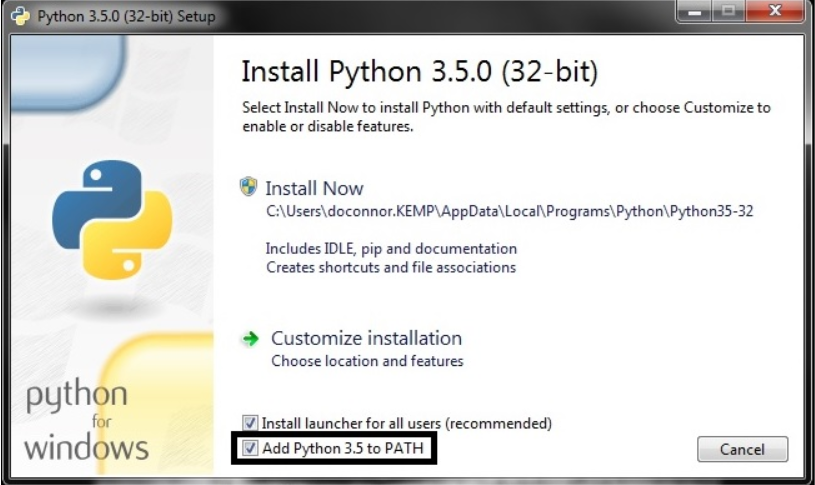
\includegraphics[width=0.95\textwidth]{images/python_installation.png}
\caption{Interface d'installation Python sur Windows}
\end{figure}

Sélectionnez "Install Now" pour une installation standard qui inclut pip, IDLE et la documentation. L'installation créé un répertoire Python dans votre dossier utilisateur et configure les associations de fichiers appropriées. Une fois l'installation terminée, vérifiez son succès en ouvrant une nouvelle invite de commandes et en exécutant \texttt{python --version}. La commande devrait afficher "Python 3.12.x" confirmant une installation réussie.

\subsubsection{Installation sur macOS}

Sur macOS, plusieurs options d'installation s'offrent aux développeurs. La méthode recommandée utilise \textbf{Homebrew}, le gestionnaire de packages populaire pour macOS. Si Homebrew n'est pas déjà installé, ouvrez Terminal et exécutez la commande d'installation officielle disponible sur \texttt{brew.sh}.

Avec Homebrew installé, l'installation de Python devient remarquablement simple. Exécutez \texttt{brew install python@3.12} dans Terminal. Homebrew gère automatiquement les dépendances, configure les liens symboliques appropriés et assure que Python est accessible globalement. Cette méthode présente l'avantage de faciliter les mises à jour futures via \texttt{brew upgrade python@3.12}.

\begin{figure}[H]
\centering
\framebox[0.9\textwidth]{
\parbox{0.85\textwidth}{
\centering
\textbf{Installation Python via Homebrew sur macOS}\\[10pt]
Terminal affiche :\\
\texttt{\$ brew install python@3.12}\\
\texttt{==> Downloading python@3.12...}\\
\texttt{==> Installing python@3.12...}\\
\texttt{==> Python has been installed at /usr/local/bin/python3.12}\\[10pt]
Installation réussie avec configuration automatique du PATH.
}
}
\caption{Installation de Python sur macOS avec Homebrew}
\end{figure}

Pour les utilisateurs préférant une installation graphique, le site python.org propose également un installateur .pkg pour macOS. Cette méthode installe Python dans \texttt{/Library/Frameworks/Python.framework} et ajoute les liens nécessaires dans \texttt{/usr/local/bin}. Quelle que soit la méthode choisie, vérifiez l'installation avec \texttt{python3.12 --version} dans Terminal.

\subsubsection{Installation sur Linux}

Les systèmes Linux offrent généralement Python préinstallé, mais souvent dans une version antérieure. L'installation de Python 3.12 varie selon la distribution, mais les principes restent similaires.

Pour les distributions basées sur \textbf{Ubuntu/Debian}, utilisez le système de gestion de packages APT. Commencez par ajouter le PPA deadsnakes qui fournit les versions récentes de Python : \texttt{sudo add-apt-repository ppa:deadsnakes/ppa}. Mettez à jour la liste des packages avec \texttt{sudo apt update}, puis installez Python avec \texttt{sudo apt install python3.12 python3.12-venv python3.12-dev}. L'inclusion des packages venv et dev est importante pour le support complet des environnements virtuels et la compilation d'extensions.

\begin{figure}[H]
\centering
\framebox[0.9\textwidth]{
\parbox{0.85\textwidth}{
\centering
\textbf{Installation Python sur Ubuntu}\\[10pt]
Terminal affiche :\\
\texttt{\$ sudo add-apt-repository ppa:deadsnakes/ppa}\\
\texttt{\$ sudo apt update}\\
\texttt{\$ sudo apt install python3.12 python3.12-venv python3.12-dev}\\
\texttt{Setting up python3.12 (3.12.x-1) ...}\\[10pt]
Configuration des alternatives Python pour définir la version par défaut.
}
}
\caption{Installation de Python sur Ubuntu Linux}
\end{figure}

Pour les distributions basées sur \textbf{Fedora/Red Hat}, utilisez DNF ou YUM selon votre système. Python 3.12 peut être installé directement depuis les dépôts officiels avec \texttt{sudo dnf install python3.12}. Les distributions entreprise comme RHEL peuvent nécessiter l'activation de dépôts supplémentaires ou la compilation depuis les sources.

\subsection{Installation de Poetry}

\textbf{Poetry} révolutionne la gestion des dépendances Python en offrant une approche moderne et déterministe. Contrairement à pip et requirements.txt traditionnels, Poetry gère automatiquement les environnements virtuels, résout les conflits de dépendances et maintient un fichier de verrouillage garantissant la reproductibilité des installations.

L'installation de Poetry utilise un script d'installation officiel qui détecte automatiquement votre système et configure Poetry de manière optimale. Sur \textbf{macOS et Linux}, ouvrez un terminal et exécutez la commande curl pour télécharger et exécuter le script d'installation. Le script crée un répertoire Poetry dans votre dossier home, installe Poetry de manière isolée et configure votre shell pour inclure Poetry dans le PATH.

\begin{figure}[H]
\centering
\framebox[0.9\textwidth]{
\parbox{0.85\textwidth}{
\centering
\textbf{Installation de Poetry}\\[10pt]
\texttt{\$ curl -sSL https://install.python-poetry.org | python3 -}\\[5pt]
\texttt{Retrieving Poetry metadata...}\\
\texttt{Installing Poetry (1.7.0)}\\
\texttt{Poetry installed successfully!}\\[5pt]
\texttt{Add Poetry to PATH:}\\
\texttt{export PATH="\$HOME/.local/bin:\$PATH"}
}
}
\caption{Installation automatisée de Poetry}
\end{figure}

Sur \textbf{Windows}, l'installation utilise PowerShell avec des privilèges administrateur. Le script PowerShell télécharge Poetry, l'installe dans le profil utilisateur et configure automatiquement les variables d'environnement Windows. Après l'installation, une nouvelle session PowerShell est nécessaire pour que les changements de PATH prennent effet.

La configuration post-installation de Poetry mérite une attention particulière. Exécutez \texttt{poetry config virtualenvs.in-project true} pour configurer Poetry à créer les environnements virtuels dans le répertoire du projet. Cette configuration facilite la gestion des environnements et l'intégration avec les IDE. Vérifiez l'installation avec \texttt{poetry --version} qui devrait afficher la version installée.

Poetry offre des fonctionnalités avancées qui simplifient significativement le workflow de développement. La commande \texttt{poetry install} lit le fichier \texttt{pyproject.toml}, crée automatiquement un environnement virtuel si nécessaire, et installe toutes les dépendances avec les versions exactes spécifiées dans \texttt{poetry.lock}. Cette approche élimine les problèmes classiques de "ça marche sur ma machine" en garantissant que tous les développeurs utilisent exactement les mêmes versions de packages.

\subsection{Installation de Git}

\textbf{Git} constitue l'outil fondamental pour la gestion de versions et la collaboration sur le projet Agriculture Cameroun. Son installation correcte et sa configuration appropriée sont essentielles pour contribuer efficacement au projet.

Sur \textbf{Windows}, Git pour Windows (Git Bash) fournit non seulement Git mais aussi un environnement shell Unix-like précieux. Téléchargez l'installateur depuis \texttt{\href{https://git-scm.com/download/win}{git-scm.com}} et lancez-le. Durant l'installation, plusieurs choix importants se présentent. 
\begin{itemize}
    \item Pour l'éditeur par défaut, sélectionnez votre éditeur préféré (VS Code est recommandé si installé). Pour l'ajustement du PATH, choisissez "Git from the command line and also from 3rd-party software" pour une intégration maximale.
    \item Pour le terminal, optez pour "Use MinTTY (the default terminal of MSYS2)" pour une expérience de ligne de commande améliorée.
    \item Pour la gestion des fins de ligne, sélectionnez "Checkout Windows-style, commit Unix-style line endings" pour assurer la compatibilité multiplateforme.
\end{itemize}

\begin{figure}[H]
\centering
\framebox[0.9\textwidth]{
\parbox{0.85\textwidth}{
\centering
\textbf{Configuration Git pour Windows}\\[10pt]
Options critiques durant l'installation :\\[5pt]
✓ Use Visual Studio Code as Git's default editor\\
✓ Git from the command line and 3rd-party software\\
✓ Checkout Windows-style, commit Unix-style endings\\
✓ Use MinTTY (Git Bash terminal)\\
✓ Enable file system caching
}
}
\caption{Options d'installation recommandées pour Git sur Windows}
\end{figure}

Sur \textbf{macOS}, Git peut être installé via Homebrew avec \texttt{\textbf{brew install git}} ou via les Xcode Command Line Tools avec \textbf{\textit{xcode-select --install}}. La méthode Homebrew est préférée car elle facilite les mises à jour futures et installe la version la plus récente de Git.

Sur \textbf{Linux}, Git est disponible dans les dépôts officiels de toutes les distributions majeures. Pour Ubuntu/Debian, utilisez \texttt{sudo apt install git}. Pour Fedora, \texttt{sudo dnf install git}. Ces commandes installent Git avec toutes ses dépendances et outils associés.

Après l'installation, la \textbf{configuration initiale de Git} est cruciale. Configurez votre identité globale avec \texttt{git config --global user.name "Votre Nom"} et \texttt{git config --global user.email "votre.email@example.com"}. Ces informations sont attachées à chaque commit que vous créez. Configurez également des alias utiles comme \texttt{git config --global alias.st status} pour accélérer les commandes fréquentes.

Pour le projet Agriculture Cameroun, configurez Git pour gérer correctement les fins de ligne multiplateformes avec \texttt{git config --global core.autocrlf true} sur Windows ou \texttt{git config --global core.autocrlf input} sur macOS/Linux. Cette configuration prévient les problèmes de fins de ligne lors de la collaboration entre développeurs utilisant différents systèmes d'exploitation.

\subsection{Configuration des clés API (Google Gemini)}

L'accès à l'API Google Gemini constitue le cœur de l'intelligence du système Agriculture Cameroun. La configuration correcte et sécurisée des clés API est donc critique pour le fonctionnement du système.

Pour obtenir une clé API Gemini, naviguez vers \texttt{makersuite.google.com/app/apikey}. Connectez-vous avec votre compte Google et créez un nouveau projet si nécessaire. Google AI Studio propose un généreux quota gratuit suffisant pour le développement et les tests. Cliquez sur "Create API Key" et copiez immédiatement la clé générée dans un endroit sûr - elle ne sera plus affichée après fermeture de la fenêtre.

\begin{figure}[H]
\centering
\framebox[0.9\textwidth]{
\parbox{0.85\textwidth}{
\centering
\textbf{Configuration de la clé API Gemini}\\[10pt]
Fichier \texttt{.env} à la racine du projet :\\[5pt]
\texttt{GEMINI\_API\_KEY=AIzaSy...votre\_cle\_api\_ici}\\
\texttt{DEFAULT\_REGION=Centre}\\
\texttt{DEFAULT\_LANGUAGE=fr}\\
\texttt{LOG\_LEVEL=INFO}\\[5pt]
⚠️ Ne jamais commiter ce fichier dans Git !
}
}
\caption{Configuration sécurisée des variables d'environnement}
\end{figure}

La \textbf{gestion sécurisée des clés API} est primordiale. Créez un fichier \texttt{.env} à la racine du projet (en copiant \texttt{.env.example} fourni). Ce fichier contient toutes les variables d'environnement sensibles. Assurez-vous que \texttt{.env} est listé dans \texttt{.gitignore} pour éviter de l'exposer accidentellement dans le contrôle de version. Le fichier \texttt{.env.example} sert de template documenté sans contenir de vraies clés.

Les \textbf{bonnes pratiques de sécurité} incluent la rotation régulière des clés API, l'utilisation de clés différentes pour le développement et la production, et la restriction des clés API aux domaines ou adresses IP spécifiques quand possible. Google Cloud Console permet de configurer ces restrictions pour minimiser les risques en cas de compromission d'une clé.

Pour les \textbf{environnements de production}, considérez l'utilisation de services de gestion de secrets comme Google Secret Manager ou HashiCorp Vault plutôt que des fichiers \texttt{.env}. Ces services offrent une gestion centralisée, l'audit des accès et la rotation automatique des secrets.

La \textbf{validation de la configuration} peut être effectuée en exécutant le script de test fourni : \texttt{python scripts/test\_api\_connection.py}. Ce script vérifie que la clé API est valide, que les quotas sont suffisants et que la connexion aux services Google est opérationnelle. En cas d'erreur, le script fournit des messages diagnostiques détaillés pour faciliter le dépannage.

\section{Structure du Projet}

\subsection{Organisation des dossiers}

La structure du projet Agriculture Cameroun reflète une architecture modulaire soigneusement conçue pour faciliter la navigation, la maintenance et l'extension du système. Cette organisation hiérarchique sépare clairement les responsabilités tout en maintenant une cohésion logique entre les composants.

\begin{figure}[H]
\centering
\fbox{
\begin{minipage}{0.9\textwidth}
\footnotesize
\begin{forest}
for tree={
    font=\ttfamily,
    grow'=0,
    child anchor=west,
    parent anchor=south,
    anchor=west,
    calign=first,
    edge path={
        \noexpand\path [draw, \forestoption{edge}]
        (!u.south west) +(7.5pt,0) |- (.child anchor)\forestoption{edge label};
    },
    before typesetting nodes={
        if n=1
            {insert before={[,phantom]}}
            {}
    },
    fit=band,
    before computing xy={l=15pt},
}
[agriculture\_cameroun/ \textcolor{gray}{\textit{Package principal}}
    [\_\_init\_\_.py \textcolor{gray}{\textit{Init package}}]
    [agent.py \textcolor{gray}{\textit{Agent coordinateur}}]
    [prompts.py \textcolor{gray}{\textit{Instructions}}]
    [tools.py \textcolor{gray}{\textit{Communication}}]
    [config.py \textcolor{gray}{\textit{Configuration}}]
    [sub\_agents/ \textcolor{gray}{\textit{Agents spécialisés}}
        [\_\_init\_\_.py \textcolor{gray}{\textit{Exports}}]
        [weather/ \textcolor{gray}{\textit{Météorologique}}
            [\_\_init\_\_.py]
            [agent.py \textcolor{gray}{\textit{Logique météo}}]
            [prompts.py \textcolor{gray}{\textit{Instructions}}]
            [tools.py \textcolor{gray}{\textit{Outils météo}}]
        ]
        [crops/ \textcolor{gray}{\textit{Cultures}}
            [\_\_init\_\_.py]
            [agent.py]
            [prompts.py]
            [tools.py]
        ]
        [health/ \textcolor{gray}{\textit{Santé plantes}}
            [\_\_init\_\_.py]
            [agent.py]
            [prompts.py]
            [tools.py]
        ]
        [economic/ \textcolor{gray}{\textit{Économique}}
            [\_\_init\_\_.py]
            [agent.py]
            [prompts.py]
            [tools.py]
        ]
        [resources/ \textcolor{gray}{\textit{Ressources}}
            [\_\_init\_\_.py]
            [agent.py]
            [prompts.py]
            [tools.py]
        ]
    ]
    [utils/ \textcolor{gray}{\textit{Utilitaires}}
        [\_\_init\_\_.py]
        [data.py \textcolor{gray}{\textit{Données agricoles}}]
        [utils.py \textcolor{gray}{\textit{Fonctions auxiliaires}}]
    ]
    [tests/ \textcolor{gray}{\textit{Tests}}
        [\_\_init\_\_.py]
        [test\_agents.py \textcolor{gray}{\textit{Tests agents}}]
    ]
]
\end{forest}
\end{minipage}
}
\caption{Structure réelle du projet Agriculture Cameroun avec Google ADK}
\label{fig:agriculture_structure_real}
\end{figure}
\begin{figure}[H]
\centering
\fbox{
\begin{minipage}{0.9\textwidth}
\footnotesize
\begin{forest}
for tree={
    font=\ttfamily,
    grow'=0,
    child anchor=west,
    parent anchor=south,
    anchor=west,
    calign=first,
    edge path={
        \noexpand\path [draw, \forestoption{edge}]
        (!u.south west) +(7.5pt,0) |- (.child anchor)\forestoption{edge label};
    },
    before typesetting nodes={
        if n=1
            {insert before={[,phantom]}}
            {}
    },
    fit=band,
    before computing xy={l=15pt},
}
[projet\_racine/ \textcolor{gray}{\textit{Dossier racine}}
    [agriculture\_cameroun/ \textcolor{gray}{\textit{Package principal}}
        [examples/ \textcolor{gray}{\textit{Exemples}}
            [demo\_cli.py \textcolor{gray}{\textit{Demo CLI}}]
            [usage\_examples.py \textcolor{gray}{\textit{Exemples pratiques}}]
        ]
    ]
    [deployment/ \textcolor{gray}{\textit{Déploiement}}
        [\_\_init\_\_.py]
        [deploy.py]
    ]
    [.env.example \textcolor{gray}{\textit{Template config}}]
    [.gitignore \textcolor{gray}{\textit{Git ignore}}]
    [pyproject.toml \textcolor{gray}{\textit{Config Poetry}}]
    [Dockerfile \textcolor{gray}{\textit{Container Docker}}]
    [docker-compose.yml \textcolor{gray}{\textit{Multi-services}}]
    [setup.sh \textcolor{gray}{\textit{Install Linux/macOS}}]
    [setup.ps1 \textcolor{gray}{\textit{Install Windows}}]
    [README.md \textcolor{gray}{\textit{Doc principale}}]
    [INSTALLATION.md \textcolor{gray}{\textit{Guide install}}]
    [QUICKSTART.md \textcolor{gray}{\textit{Démarrage 5min}}]
    [USER\_GUIDE.md \textcolor{gray}{\textit{Guide utilisateur}}]
    [API\_DOCUMENTATION.md \textcolor{gray}{\textit{Doc API REST}}]
    [CONTRIBUTING.md \textcolor{gray}{\textit{Guide contribution}}]
    [FAQ.md \textcolor{gray}{\textit{Questions FAQ}}]
    [LICENSE \textcolor{gray}{\textit{Licence Apache 2.0}}]
]
\end{forest}
\end{minipage}
}
\caption{Structure complète du projet avec fichiers de configuration et documentation}
\label{fig:agriculture_structure_complete}
\end{figure}


Le \textbf{répertoire racine} contient les composants principaux du système. Le fichier \texttt{agent.py} implémente l'agent coordinateur qui route les requêtes vers les agents spécialisés. Le fichier \texttt{prompts.py} centralise les instructions de l'agent principal, tandis que \texttt{tools.py} définit les outils de communication inter-agents. Le fichier \texttt{config.py} gère la configuration globale et les modèles de données.

Le \textbf{répertoire sub\_agents} héberge les cinq agents spécialisés : \textit{weather} (météorologie), \textit{crops} (cultures), \textit{health} (santé des plantes), \textit{economic} (économie) et \textit{resources} (ressources). Chaque agent suit une structure standardisée avec trois fichiers : \texttt{agent.py} (logique principale), \texttt{prompts.py} (instructions spécialisées) et \texttt{tools.py} (outils métier).

Le \textbf{répertoire utils} contient les utilitaires partagés. Le fichier \texttt{data.py} centralise les données agricoles camerounaises (régions, cultures, prix, calendriers), tandis que \texttt{utils.py} fournit les fonctions auxiliaires communes au système.

Le \textbf{répertoire tests} implémente les tests du système avec \texttt{test\_agents.py} pour les tests unitaires des agents.

Le \textbf{répertoire examples} propose des démonstrations pratiques avec \texttt{demo\_cli.py} (interface ligne de commande interactive) et \texttt{usage\_examples.py} (exemples d'utilisation programmatique).

La \textbf{documentation} comprend plusieurs guides : \texttt{README.md} (présentation générale), \texttt{INSTALLATION.md} (installation détaillée), \texttt{QUICKSTART.md} (démarrage rapide), \texttt{USER\_GUIDE.md} (guide utilisateur) et \texttt{API\_DOCUMENTATION.md} (documentation de l'API REST).

\subsection{Fichiers de configuration importants}

Les fichiers de configuration du projet Agriculture Cameroun orchestrent le comportement du système et définissent son environnement d'exécution. Leur compréhension approfondie est essentielle pour personnaliser et déployer efficacement le système.

Le fichier \textbf{pyproject.toml} sert de manifeste central pour le projet. Ce fichier moderne remplace les traditionnels \texttt{setup.py} et \texttt{requirements.txt}, centralisant toutes les métadonnées du projet. Il définit le nom du projet, sa version, sa description et ses auteurs. La section \texttt{[tool.poetry.dependencies]} liste toutes les dépendances avec leurs contraintes de version, assurant la reproductibilité des installations. La section \texttt{[tool.poetry.dev-dependencies]} sépare clairement les outils de développement des dépendances de production. Les configurations des outils de développement (pytest, black, mypy) sont également centralisées ici, créant une source unique de vérité pour la configuration du projet.

% \begin{figure}[H]
% \centering
% \framebox[0.9\textwidth]{
% \parbox{0.85\textwidth}{
% \footnotesize
% \texttt{[tool.poetry]}\\
% \texttt{name = "agriculture-cameroun"}\\
% \texttt{version = "1.0.0"}\\
% \texttt{description = "Système multi-agents pour l'agriculture"}\\
% \texttt{authors = ["Mbassi Loic <wwwmbassiloic@gmail.com>"]}\\[5pt]
% \texttt{[tool.poetry.dependencies]}\\
% \texttt{python = ">=3.12,<3.13"}\\
% \texttt{google-generativeai = "^0.3.0"}\\
% \texttt{pydantic = "^2.0"}\\
% \texttt{python-dotenv = "^1.0.0"}\\[5pt]
% \texttt{[tool.poetry.dev-dependencies]}\\
% \texttt{pytest = "^7.4"}\\
% \texttt{black = "^23.0"}\\
% \texttt{mypy = "^1.5"}
% }
% }
% \caption{Extrait du fichier pyproject.toml}
% \end{figure}

Le fichier \textbf{.env} (et son template \texttt{.env.example}) gère les variables d'environnement sensibles et spécifiques à chaque déploiement. Au-delà de la clé API Gemini, ce fichier configure le comportement du système : région par défaut, langue d'interface, niveau de logging, timeouts des API. La séparation entre \texttt{.env} (ignoré par Git) et \texttt{.env.example} (versionné) permet de documenter les variables nécessaires sans exposer les valeurs réelles.

Le fichier \textbf{config.py} transforme les variables d'environnement en configuration Python typée et validée. Utilisant Pydantic, il définit des classes de configuration avec validation automatique, valeurs par défaut intelligentes et documentation intégrée. Cette approche centralise la configuration, facilite les tests avec des configurations alternatives et fournit une interface programmatique claire pour accéder aux paramètres.

Les fichiers \textbf{.gitignore} et \textbf{.gitattributes} contrôlent le comportement de Git. Le \texttt{.gitignore} exclut non seulement les fichiers sensibles et temporaires standards, mais aussi les artefacts spécifiques au projet comme les caches de modèles et les logs de développement. Le \texttt{.gitattributes} assure un traitement cohérent des fins de ligne entre plateformes et marque certains fichiers pour un traitement spécial lors des merges.

Le fichier \textbf{docker-compose.yml} (quand présent) définit l'architecture conteneurisée du système. Il spécifie les services, leurs dépendances, les volumes pour la persistance des données et les réseaux pour l'isolation. Cette configuration facilite le déploiement cohérent across environnements et simplifie l'onboarding de nouveaux développeurs.

\subsection{Conventions de nommage et bonnes pratiques}

Les conventions de nommage et les bonnes pratiques établies pour le projet Agriculture Cameroun assurent la cohérence, la lisibilité et la maintenabilité du code à travers toutes les contributions.

Les \textbf{conventions de nommage Python} suivent strictement PEP 8 avec quelques clarifications spécifiques au projet. Les noms de classes utilisent PascalCase (\texttt{WeatherAgent}, \texttt{CropRecommendation}), communiquant clairement leur nature d'objets. Les fonctions et méthodes emploient snake\_case (\texttt{get\_weather\_forecast}, \texttt{analyze\_soil\_data}), avec des verbes d'action pour les fonctions qui effectuent des opérations. Les constantes utilisent SCREAMING\_SNAKE\_CASE (\texttt{MAX\_RETRY\_ATTEMPTS}, \texttt{DEFAULT\_TIMEOUT}), les distinguant visuellement des variables. Les modules et packages maintiennent snake\_case minuscule, reflétant la convention Python standard.

La \textbf{structure des imports} suit un ordre strict pour améliorer la lisibilité. Les imports de la bibliothèque standard viennent en premier, suivis des imports de packages tiers, puis des imports locaux du projet. Au sein de chaque groupe, les imports sont ordonnés alphabétiquement. Les imports absolus sont préférés aux imports relatifs pour la clarté, sauf within un même package où les imports relatifs peuvent améliorer la cohésion.

Les \textbf{docstrings} constituent une exigence non négociable pour toutes les fonctions publiques, classes et modules. Le format Google-style est adopté pour sa lisibilité et sa compatibilité avec les outils de documentation automatique. Chaque docstring inclut une description concise, la documentation des paramètres avec leurs types, la valeur de retour et ses types, et les exceptions potentielles. Les exemples d'utilisation sont encouragés pour les fonctions complexes.

% \begin{figure}[H]
% \centering
% \framebox[0.9\textwidth]{
% \parbox{0.85\textwidth}{
% \footnotesize
% \begin{verbatim}
% def analyze_crop_suitability(
%     region: str,
%     crop_type: str,
%     soil_data: dict[str, float]
% ) -> CropRecommendation:
%     """Analyse l'adéquation d'une culture pour une région.

%     Args:
%         region: Code de la région camerounaise (ex: 'Centre')
%         crop_type: Type de culture à analyser (ex: 'cacao')
%         soil_data: Données du sol (pH, N, P, K, etc.)

%     Returns:
%         CropRecommendation avec score et recommandations

%     Raises:
%         ValueError: Si la région ou culture est invalide
%         DataError: Si les données du sol sont incomplètes
%     """
% \end{verbatim}
% }
% }
% \caption{Exemple de docstring suivant les conventions du projet}
% \end{figure}

La \textbf{gestion des erreurs} privilégie la spécificité et l'information. Les exceptions personnalisées sont définies pour les erreurs métier spécifiques (\texttt{InvalidCropError}, \texttt{WeatherDataUnavailableError}). Les messages d'erreur incluent suffisamment de contexte pour faciliter le débogage. Le principe "fail fast" est appliqué, validant les entrées tôt dans le flux d'exécution. Les erreurs attendues (comme les timeouts réseau) sont gérées gracieusement avec des stratégies de retry appropriées.

Les \textbf{patterns de conception} appropriés sont encouragés sans sur-ingénierie. Le pattern Strategy est utilisé pour les différents agents, permettant l'ajout facile de nouveaux agents. Le pattern Factory simplifie la création d'agents basée sur la configuration. Le pattern Observer facilite la communication asynchrone entre composants. Ces patterns sont appliqués judicieusement, seulement quand ils apportent une valeur claire.

La \textbf{gestion de la complexité} suit le principe de responsabilité unique. Les fonctions restent courtes et focalisées, idéalement sous 20 lignes. La complexité cyclomatique est maintenue basse par l'extraction de sous-fonctions et l'utilisation de structures de données appropriées. Les classes encapsulent un concept cohérent sans devenir des "god objects". Les modules regroupent des fonctionnalités liées sans créer de couplage excessif.

Les \textbf{pratiques de sécurité} sont intégrées dès la conception. Les entrées utilisateur sont systématiquement validées et assainies. Les secrets ne sont jamais codés en dur ou loggés. Les dépendances sont régulièrement auditées pour les vulnérabilités. Le principe du moindre privilège guide les permissions et accès. Les données sensibles des agriculteurs sont traitées avec le plus grand soin, suivant les principes de protection des données personnelles.
